\documentclass{beamer}

\usepackage{graphicx}

\usetheme{Boadilla}

\AtBeginSection[]{
    \begin{frame}
    \vfill
    \centering
      \usebeamerfont{title}\insertsectionhead\par%
    \vfill
    \end{frame}
}

\title{Esplorare L'API Grafica Vulkan}
\author{Emanuele Franchi}
\date{}

\begin{document}

\begin{frame}

\titlepage

\end{frame}


\section{Vulkan}
\begin{frame}
\frametitle{Vulkan Come API Grafica}
\begin{columns}

\column{.6\textwidth}

\begin{itemize}
\item Vulkan è un'API grafica cross platform di nuova generazione
\item Un'API grafica è un'interfaccia che ci permette di interagire con la GPU
\end{itemize}

\column{.2\textwidth}

\begin{figure}[ht]
    \centering
    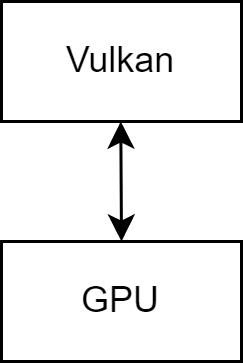
\includegraphics[scale=0.2]{images/SlidesVulkan/VulkanAPI.png}
\end{figure}

\end{columns}
\end{frame}

\begin{frame}
\frametitle{Vulkan Come Specifica}
\begin{columns}

\column{.6\textwidth}

\begin{itemize}
\item

\end{itemize}

\column{.2\textwidth}

\begin{figure}[ht]
    \centering
    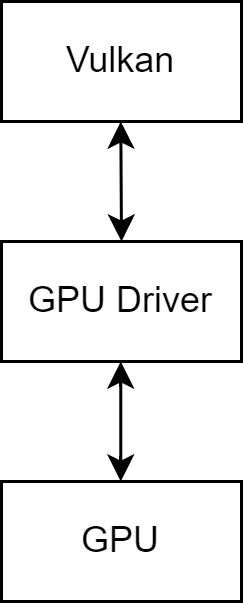
\includegraphics[scale=0.2]{images/SlidesVulkan/VulkanSpecification.png}
\end{figure}

\end{columns}
\end{frame}

\begin{frame}
\frametitle{OpenGL Pros And Cons}

\begin{itemize}
\item Predecessore di Vulkan
\item Anno di rilascio: 1992
\item Sviluppata usando come modello l'architettura delle GPU dell'epoca
\item Estesa in seguito per esporre le funzionalità delle nuove schede grafiche
\item Questo ha portato ad una complessità crescente dei driver
\item Questo causa overhead e inconsistenze tra driver diversi
\item Sviluppata quando le CPU erano prevalentemente single core
\item Sviluppata per essere usata in un contesto single threaded
\end{itemize}

\end{frame}

\begin{frame}
\frametitle{Vulkan (2)}

\begin{itemize}
\item Successore di OpenGL
\item Anno di rilascio: 2016
\item Sviluppata usando come modello l'architettura delle GPU odierne
\item Driver molto più semplici e leggeri
\item A più basso livello rispetto ad OpenGL
\item Richiede più conoscenze da parte del programmatore
\item Più verbosa rispetto ad OpenGL
\item Può risultare in performance migliori, se il programmatore la usa coscientemente
\item Sviluppata per essere usata in un contesto multithreaded
\item Essendo così nuova, le GPU meno recenti non la supportano
\end{itemize}

\end{frame}


\section{Inizializzare Vulkan}
\begin{frame}
\frametitle{Vulkan Instance}
\begin{columns}

\column{.6\textwidth}

\begin{itemize}
\item Dobbiamo creare un'istanza di Vulkan per accedere al resto dell'API
\item Quando creiamo un'istanza indichiamo i layer che vogliamo abilitare
\item I layer sono componenti opzionali
\item I layer modificano il comportamento delle funzioni dell'API
\item Per esempio, possiamo usare un layer per controllare se il nostro utilizzo dell'API non violi la specifica
\item Quando creiamo un'istanza indichiamo le estensioni d'istanza che vogliamo abilitare
\item Le estensioni aggiungono nuove funzioni all'API
\end{itemize}

\column{.4\textwidth}

\begin{figure}[ht]
    \centering
    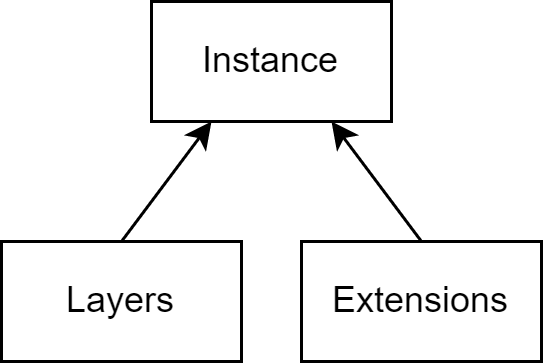
\includegraphics[scale=0.2]{images/SlidesInitializingVulkan/Instance.png}
\end{figure}

\end{columns}
\end{frame}

\begin{frame}
\frametitle{Finestra e Vulkan Presentation Surface}
\begin{columns}

\column{.6\textwidth}

\begin{itemize}
\item Creiamo una finestra usando l'API del sistema operativo
\item Creiamo una Vulkan presentation surface per interagire con la finestra creata
\end{itemize}

\column{.2\textwidth}

\begin{figure}[ht]
    \centering
    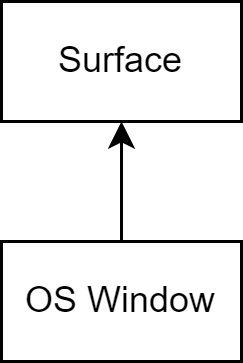
\includegraphics[scale=0.2]{images/SlidesInitializingVulkan/WindowAndSurface.png}
\end{figure}

\end{columns}
\end{frame}

\begin{frame}
\frametitle{Selezionare Un Device Fisico}

\begin{itemize}
\item Dobbiamo selezionare la GPU che andremo a utilizzare
\item Deve supportare operazioni grafiche, quindi deve avere almeno una coda che possa eseguire tali comandi
\item Deve supportare operazioni di presentazione di immagini, quindi deve avere almeno una coda che possa eseguire tali comandi
\item Deve supportare la creazione di una swapchain
\item Deve supportare almeno una modalità di presentazione compatibile con la presentation surface che abbiamo creato precedentemente
\end{itemize}

\end{frame}

\begin{frame}
\frametitle{Creare Un Device Logico}
\begin{columns}

\column{.6\textwidth}

\begin{itemize}
\item Per interagire con il device fisico selezionato, dobbiamo creare un device logico
\item Quando creiamo il device logico, indichiamo la creazione di una coda per eseguire comandi grafici, e una coda per eseguire comandi di presentazione
\item Una volta creato il device logico, possiamo ottenere le code richieste
\item Se una coda supporta sia operazioni grafiche che di presentazione, possiamo usarla singolarmente
\end{itemize}

\column{.2\textwidth}

\begin{figure}[ht]
    \centering
    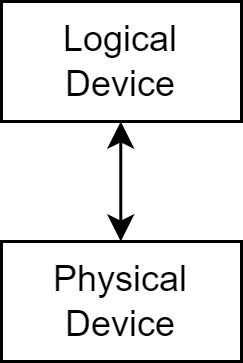
\includegraphics[scale=0.2]{images/SlidesInitializingVulkan/LogicalDevice.png}
\end{figure}

\end{columns}
\end{frame}

\begin{frame}
\frametitle{Creare Una Swapchain}
\begin{columns}

\column{.6\textwidth}

\begin{itemize}
\item Una volta creato un device logico, lo possiamo utilizzare per creare una swapchain
\item Dobbiamo creare una swapchain per presentare immagini sulla presentation surface
\item Una swapchain crea e gestisce le immagini che saranno presentate
\item Tramite la swapchain dobbiamo specificare la modalità di presentazione che verrà usata dal presentation engine del sistema operativo
\end{itemize}

\column{.2\textwidth}

\begin{figure}[ht]
    \centering
    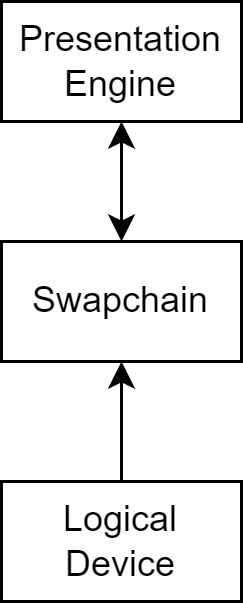
\includegraphics[scale=0.2]{images/SlidesInitializingVulkan/Swapchain.png}
\end{figure}

\end{columns}
\end{frame}


\end{document}
